\begin{abstract}
Pronunciation assessment depends on expert-scored speech. PAL, a Panel of Artificial Listeners, measures how recoverable a known
prompt is from a learner's reading with heterogeneous recognizers: each recognizer's phoneme error against the prompt is a
measurement, and the equal-weight mean over \N{Panel} recognizers admitted
by an a-priori rule is the readout. No panel weight or score parameter is
fitted to human ratings; ratings serve only development and validation.
Design was fixed on the \so{} training split; five primary confirmatory comparisons were pre-specified and tested once
after protocol commitment.
PAL exceeds the best single
recognizer on the held-out test split ($\Delta r=\N{TestDelta}$
[\N{TestDeltaLo}, \N{TestDeltaHi}]), is segmental rather than prosodic on ERJ, replicates on EpaDB, correlates
with human word recognition on ALLSSTAR ($r=\N{All}$), and tracks Mandarin tone above consonant ratings.
High-error recognizers retain most signal; none of the tested
aggregation rules beats the mean. The scale is relative; grades need anchors.
\end{abstract}
\begin{keywords}
pronunciation assessment, speech recognition, intelligibility, phoneme error rate, pre-specified protocol
\end{keywords}

\section{Introduction}
\label{sec:intro}
Supervised assessors such as GOPT and HMamba learn multiple rating
aspects from expert-scored speech \cite{gong2022,chao2025hmamba}, and every new learner population or language brings the same labeling
cost \cite{zhang2021speechocean}. We ask a measurement
question instead of a prediction question: can the errors that a set of
dissimilar recognizers make on a known prompt serve as a rating-free
measurement of how recoverable a learner's pronunciation is, and what does
that measurement correspond to in human judgment?

Words are easier for some listeners to recover than for others
\cite{bent2003}, and intelligibility is a teaching target distinct from
nativelikeness \cite{munro1995,levis2005}; recognizers that differ in
architecture, training data, and decoding are probes with different
failure modes. ASR-derived measures have long been associated with
pronunciation ratings
\cite{neumeyer2000,cucchiarini2000}, single-recognizer error features enter supervised assessors
\cite{do2024mixup}, ASR scores are combined with acoustic predictors of
accentedness and comprehensibility \cite{dong2026accent}, and
within-family Whisper ensembles feed supervised intelligibility predictors
\cite{jin2025chorus,jin2026stereo}. A recognizer that recovers accented speech
almost perfectly, however, has little variation left with which to rank
pronunciations \cite{won2025}. PAL is not an ensemble predictor but a pre-specified measurement
instrument in which each recognizer's errors are one repeated measurement
of the same utterance: the errors themselves are the measurement, the
panel is defined by an inclusion rule rather than by performance, and
nothing is fitted to ratings.

The contribution is PAL, a Panel of Artificial Listeners, as a measurement
instrument with a pre-specified validity study. PAL differs from recognition ensembles in objective and construction: it
does not combine hypotheses to improve transcription, and it fits no
predictor to ratings; recognizer-specific errors are repeated measurements
of prompt recoverability, and the instrument is validated across learner
populations, languages, and a direct human intelligibility criterion. Section~\ref{sec:method}
fixes the readout, the panel rule, seven hypotheses, and an unlock order for
five corpora before any confirmatory data are read.  Code, inventories, and the analysis plan are
public.\footnote{\small \url{https://github.com/mnaoizy/pal-panel}}

\section{Measurement design}
\label{sec:method}
\subsection{Readout}
For utterance $u$ with prompt $t$, listener $k$ returns a hypothesis
$h_k(u)$. Prompt and hypothesis pass through the same normalization
(lowercasing, ASCII punctuation other than apostrophes to spaces, digits to
spoken names) and the same \texttt{g2p\_en} conversion to stress-stripped
ARPAbet. The phoneme error rate $e_k(u)\in[0,1]$ is the Levenshtein distance
divided by the reference length, capped at one; an empty hypothesis scores
one. Phone recognizers are compared directly with eSpeak reference phones,
without inventory mapping. The readout is
\begin{equation}
p(u)=-\frac{1}{K}\sum_{k=1}^{K}e_k(u),
\label{eq:panel}
\end{equation}
an equal-weight mean over the $K$ admitted listeners; larger $p(u)$ means
greater recoverability. For Mandarin, characters are simplified and pinyin conversion
yields separate syllable-base and tone sequences, giving character, base,
and tone error channels. Tones are canonical lexical tones from pinyin
conversion with the neutral tone as a fifth category; tone sandhi and
polyphonic characters are not modeled.

\subsection{Panel rule}
The candidate inventory is the set of recognizer configurations whose
transcripts of these corpora existed before this study. It was assembled
in earlier work that inspected \so{} correlations; the admission rule
below does not, no candidate was added or removed for this study, and the
excluded configurations are released with their reasons. Admission is decided before any result is seen:
openly downloadable weights; support for the target language or a universal phone inventory;
one configuration per acoustic checkpoint, so decoder variants of an
admitted checkpoint are excluded; no artificially degraded inputs; no
configuration whose checkpoint identity is undocumented. Every
configuration that passes is admitted, and none is removed for performance.
Applied to the available English transcripts this admits \N{Panel}
listeners in \N{Families} families (Table~\ref{tab:panel}); the Mandarin
panel has \N{OmListeners}.

\begin{table}[!ht]
\centering
\caption{English panel by family with mean phoneme error on the \so{}
training split. Empty outputs (moonshine, \N{MoonEmpty}\%) score as
full deletion; checkpoint identifiers, decoder settings, and transcript
hashes are in the released inventory.}
\label{tab:panel}
\vspace{3pt}
\small
\begin{minipage}{\columnwidth}\sloppy
\textbf{GMM--HMM}: \textsf{sphinx-enus} (\N{ErrSphinxEnus}).
\textbf{Kaldi hybrid}: \textsf{vosk-small} (\N{ErrVoskSmall}).
\textbf{Convolutional CTC}: \textsf{jasper} (\N{ErrJasper}), \textsf{quartznet} (\N{ErrQuartznet}).
\textbf{Self-supervised CTC, LibriSpeech}: \textsf{wav2vec2-base} (\N{ErrWav2vec2Base}), \textsf{w2v2-large-lv60} (\N{ErrW2v2LargeLv60}), \textsf{wav2vec2-robust} (\N{ErrWav2vec2Robust}), \textsf{hubert-large} (\N{ErrHubertLarge}), \textsf{wavlm-large} (\N{ErrWavlmLarge}).
\textbf{Self-supervised CTC, other domains}: \textsf{w2v2-xlsr-cv} (\N{ErrW2v2XlsrCv}), \textsf{xlsr-1b-cv} (\N{ErrXlsr1bCv}), \textsf{w2v2-swbd} (\N{ErrW2v2Swbd}), \textsf{atc-w2v2} (\N{ErrAtcW2v2}), \textsf{atc-xlsr} (\N{ErrAtcXlsr}).
\textbf{Whisper}: \textsf{tiny} (\N{ErrTiny}), \textsf{tiny.en} (\N{ErrTinyEn}), \textsf{base.en} (\N{ErrBaseEn}), \textsf{small.en} (\N{ErrSmallEn}), \textsf{distil-small.en} (\N{ErrDistilSmallEn}), \textsf{distil-large-v3} (\N{ErrDistilLargeV3}), \textsf{crisperwhisper} (\N{ErrCrisperwhisper}).
\textbf{Other encoder--decoders}: \textsf{canary-1b} (\N{ErrCanary1b}), \textsf{seamless-m4t-v2} (\N{ErrSeamlessM4tV2}), \textsf{moonshine-base} (\N{ErrMoonshineBase}).
\textbf{Transducer}: \textsf{parakeet} (\N{ErrParakeet}).
\textbf{Speech LLM}: \textsf{qwen2audio} (\N{ErrQwen2audio}).
\textbf{Phone recognizers}: \textsf{espeak-phone} (\N{ErrEspeakPhone}), \textsf{allosaurus-eng} (\N{ErrAllosaurusEng}).
\end{minipage}
\end{table}

\subsection{Hypotheses and protocol}
Seven hypotheses were written before analysis; five (H1, H2, H4, H5, H6)
form the primary confirmatory tests, one per corpus, and H3 and H7 are
pre-specified secondary composition analyses. H1: the readout correlates
with pronunciation-quality ratings. H2: the panel exceeds the best single
listener, chosen on development data. H3: cross-family panels exceed
single-family panels of equal size and matched strength. H4: the readout
associates more with segmental than with prosodic ratings. H5: it correlates
with human word recognition. H6: the tone channel tracks tone ratings more
than consonant ratings. H7: high-error listeners alone retain signal.

The \so{} training split (\N{SoTrain} utterances, \N{SoTrainSpk} speakers)
was the only development data: readout, panel rule, statistics, and every
comparator were fixed there. Confirmatory data were then unlocked once each in a fixed order, \so{}
test, ERJ, EpaDB, ALLSSTAR, OMPAL, each with one pre-specified primary
comparison and a decision rule, after the analysis plan was committed to
version control. This guarantees that no confirmatory analysis was inspected before
protocol commitment; it does not imply first exposure to these public
corpora, which we had used before.\footnote{\small Analysis-plan commit \texttt{0525275} (2026-09-13
20:44 JST) in the released repository; the confirmatory results were
committed afterwards. The plan was not lodged with an external registry.} Correlations are Pearson
$r$ with \N{Boot} speaker-clustered (talker-clustered for ALLSSTAR)
percentile bootstrap resamples, seed \N{Seed}; paired differences use the
same resamples. Secondary analyses are exploratory and uncorrected.
The comparators fixed on the training split are the single listener
\textsf{hubert-large}, the \N{WeakN} highest-error listeners (weak third),
and \N{Draws} cross-family draws matched to the \N{WhisK} Whisper
listeners in mean error ($\pm0.03$) and mean single-listener correlation
($\pm0.02$).

\section{Data}
\label{sec:data}
\so{} \cite{zhang2021speechocean} has \N{SoTrain} training and \N{SoTest}
test utterances from disjoint Mandarin-L1 speakers with five-rater consensus
ratings of accuracy, completeness, fluency, prosody, and total.
ERJ \cite{minematsu2004} has \N{ErjN} sentences from \N{ErjSpk} Japanese-L1
speakers, rated for segmental quality, rhythm, and intonation on disjoint
utterances of the same speakers. EpaDB \cite{vidal2019} has \N{EpaN}
utterances from \N{EpaSpk} Argentinian-Spanish-L1 speakers with a
holistic pronunciation-quality phrase score (annotator 1); segmental
specificity is tested on ERJ, not here. ALLSSTAR \cite{bradlow2010allsstar,kim2025intelligibility}
supplies \N{AllUtt} clean HINT sentences from \N{AllTalkers} talkers of 21
first languages; the criterion is each talker's mean word-recognition
accuracy by L1-English listeners across quiet and noise conditions. OMPAL
\cite{hsieh2025ompal} has \N{OmN} Mandarin utterances from \N{OmSpk}
French-L1 learners with word-level tone and consonant ratings; its
transcripts come from a re-decode that kept the text.
All transcripts predate this study; files, listener identities, row
counts, and empty-output counts are catalogued in the released inventory.

\section{Results}
\label{sec:results}
\subsection{Development split}
On the training split the panel correlates with accuracy at
$r=\N{DevAcc}$ [\N{DevAccLo}, \N{DevAccHi}] and with completeness at only
\N{DevComp}; the best single listener, \textsf{hubert-large}, reaches
\N{DevBestR}. Random subsets of one, four, eight, and all \N{Panel}
listeners average \N{Curve1}, \N{Curve4}, \N{Curve8}, and \N{Curve28}.
 The weak third alone reaches \N{DevWeakR},
above the strong third (\N{DevStrongR}), and matched cross-family panels of
seven exceed the seven Whisper listeners by \N{DevWhisDelta}
[\N{DevWhisDeltaLo}, \N{DevWhisDeltaHi}]. Figure~\ref{fig:listeners} places every listener by
error rate and rating correlation: recognition accuracy does not order the
listeners as measurement probes, and the panel mean sits above all of them.
These observations fixed the comparators; nothing else was changed.
\begin{figure}[t]
\centering
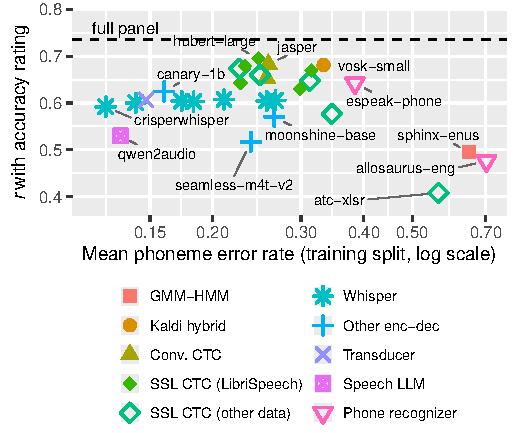
\includegraphics[width=\columnwidth]{figures/listeners.pdf}
\caption{Each admitted listener on the \so{} training split: mean phoneme
error rate (log scale) against correlation with the accuracy rating, by
family; selected listeners are labeled (all are named in
Table~\ref{tab:panel}). The dashed line is the equal-weight PAL panel.}
\label{fig:listeners}
\end{figure}

\subsection{Pre-specified confirmations}
\begin{table}[!ht]
\centering
\caption{Pre-specified primary comparisons, each run once after protocol
commitment (SO762 = \so{}); \N{Boot}-resample clustered 95\% intervals. All five
decision rules (interval excludes zero) are met.}
\label{tab:confirm}
\small
\setlength{\tabcolsep}{3pt}
\setlength{\tabcolsep}{2pt}
\begin{tabularx}{\columnwidth}{@{}lXl@{}}
\toprule
Data & Primary comparison & Result\\
\midrule
SO762 test & H2: PAL $-$ best single, accuracy & $\N{TestDelta}$ [$\N{TestDeltaLo}$, $\N{TestDeltaHi}$]\\
ERJ & H4: segmental $-$ rhythm & $\N{ErjSegRhy}$ [$\N{ErjSegRhyLo}$, $\N{ErjSegRhyHi}$]\\
EpaDB & H1: $r$, phrase score & \N{Epa} [\N{EpaLo}, \N{EpaHi}]\\
ALLSSTAR & H5: talker $r$, word recovery & \N{All} [\N{AllLo}, \N{AllHi}]\\
OMPAL & H6: tone $-$ consonant & $\N{OmDelta}$ [$\N{OmDeltaLo}$, $\N{OmDeltaHi}$]\\
\bottomrule
\end{tabularx}
\end{table}
Table~\ref{tab:confirm} lists the five primary comparisons. On the \so{}
test split PAL reaches accuracy $r=\N{TestAcc}$
[\N{TestAccLo}, \N{TestAccHi}] against \N{TestHubert} for the fixed single
listener, and \N{TestFlu}, \N{TestPros}, \N{TestTotal}, and \N{TestComp}
for fluency, prosody, total, and completeness. Table~\ref{tab:position}
places this beside published systems: supervised predictors trained on the
benchmark's ratings score higher, whereas PAL, which uses no ratings, is
comparable to published rating-free baselines and to inter-rater
agreement.
\begin{table}[!ht]
\centering
\caption{Accuracy correlation on the \so{} test split. Published values
are quoted, not reproduced; human agreement uses the released five-rater
scores.}
\label{tab:position}
\vspace{2pt}
\small
\setlength{\tabcolsep}{3pt}
\begin{tabularx}{\columnwidth}{@{}Xc@{}}
\toprule
System & Acc.\ $r$\\
\midrule
\multicolumn{2}{@{}l}{\itshape Supervised on \so{} ratings (published)}\\
GOPT \cite{gong2022} & \N{PubGopt}\\
HMamba \cite{chao2025hmamba} & \N{PubHmamba}\\
\multicolumn{2}{@{}l}{\itshape Without expert ratings (published)}\\
Transcript-guided DTW distance \cite{sara2026surprisal} & \N{PubDtw}\\
TextPA, Gemini-2.0-flash \cite{chen2025textpa} & \N{PubTextpa}\\
\multicolumn{2}{@{}l}{\itshape Without expert ratings (this work, pre-specified)}\\
Best single listener, \textsf{hubert-large} & \N{TestHubert}\\
PAL, equal-weight mean of \N{Panel} & \N{TestPanelAcc}\\
\multicolumn{2}{@{}l}{\itshape Human raters}\\
Mean pairwise agreement (five raters) & \N{HumPair}\\
Each rater versus mean of the other four & \N{HumRest}\\
\bottomrule
\end{tabularx}
\end{table} On ERJ the panel correlates with
segmental quality at \N{ErjSeg} [\N{ErjSegLo}, \N{ErjSegHi}] but with rhythm
at \N{ErjRhy} and intonation at \N{ErjInt}; the segmental-minus-intonation difference is $\N{ErjSegInt}$
[$\N{ErjSegIntLo}$, $\N{ErjSegIntHi}$]. On EpaDB the panel
exceeds \textsf{hubert-large} by $\N{EpaDelta}$
[$\N{EpaDeltaLo}$, $\N{EpaDeltaHi}$] and reaches \N{EpaSpkR} at the
speaker level.

\begin{figure}[t]
\centering
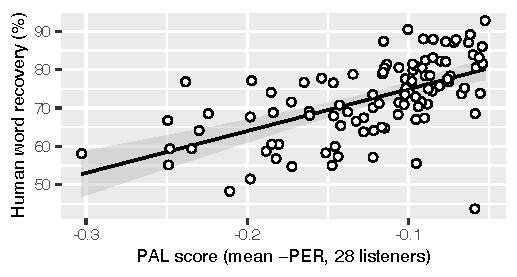
\includegraphics[width=.8\columnwidth]{figures/allsstar.pdf}
\caption{Panel score and human word recognition for \N{AllTalkers}
ALLSSTAR talkers ($r=\N{All}$ [\N{AllLo}, \N{AllHi}]). Each point is a
talker; the line is the least-squares fit.}
\label{fig:allsstar}
\end{figure}
ALLSSTAR replaces expert ratings with the words that human listeners
actually recovered; each talker's \N{AllUttPer} utterance scores are
averaged before correlation (Fig.~\ref{fig:allsstar}). The panel exceeds the fixed
single listener (\N{AllHubert}) by $\N{AllDelta}$
[$\N{AllDeltaLo}$, $\N{AllDeltaHi}$]; its margin over the seven Whisper
listeners (\N{AllWhis}) is $\N{AllWhisDelta}$
[$\N{AllWhisDeltaLo}$, $\N{AllWhisDeltaHi}$]. On OMPAL the tone channel
correlates with tone ratings at \N{OmTone} [\N{OmToneLo}, \N{OmToneHi}] and
with consonant ratings at \N{OmToneCons}, whereas the syllable-base
channel gives \N{OmBaseTone} and \N{OmBaseCons}. Counting tone errors only on syllables
whose base pinyin matches the reference raises the tone correlation to
\N{OmMatched} [\N{OmMatchedLo}, \N{OmMatchedHi}] with consonant at
\N{OmMatchedCons}, so the tone signal is not a by-product of base-syllable
errors.

\subsection{Composition and aggregation}
\begin{table}[!ht]
\centering
\caption{Secondary analyses on the \so{} test split (accuracy); $\Delta$
is paired against the comparator named in the row. Comparators were fixed
on the training split.}
\label{tab:secondary}
\small
\setlength{\tabcolsep}{3pt}
\begin{tabularx}{\columnwidth}{@{}Xcc@{}}
\toprule
Configuration & $r$ & $\Delta$ [interval]\\
\midrule
PAL, equal-weight mean & \N{TestPanelAcc} & ---\\
Weak third (\N{WeakN}) vs.\ \textsf{hubert-large} & \N{TestWeak} & $\N{TestWeakDelta}$ [$\N{TestWeakDeltaLo}$, $\N{TestWeakDeltaHi}$]\\
Whisper panel (\N{WhisK}) & \N{TestWhisSame} & ---\\
Matched cross-family (\N{Draws} draws) vs.\ Whisper & \N{TestWhisCross} & $\N{TestWhisDelta}$ [$\N{TestWhisDeltaLo}$, $\N{TestWhisDeltaHi}$]\\
Median over listeners vs.\ PAL & \N{AggMedianR} & $\N{AggMedianDelta}$ [$\N{AggMedianDeltaLo}$, $\N{AggMedianDeltaHi}$]\\
Minimum error per utterance vs.\ PAL & \N{AggMinR} & $\N{AggMinDelta}$ [$\N{AggMinDeltaLo}$, $\N{AggMinDeltaHi}$]\\
Inverse training-error weights vs.\ PAL & \N{AggInvR} & $\N{AggInvDelta}$ [$\N{AggInvDeltaLo}$, $\N{AggInvDeltaHi}$]\\
\bottomrule
\end{tabularx}
\end{table}
Table~\ref{tab:secondary} answers whether the instrument is more than an
average of many recognizers. Every matched cross-family draw scores above
the Whisper panel on the test split (\N{TestWhisFrac}\% of draws), but on
ALLSSTAR the margin over Whisper includes zero, so family breadth is
supported on the development benchmark and not established on the external
criterion. The weak third alone reaches \N{TestWeak}
[\N{TestWeakLo}, \N{TestWeakHi}], close to the fixed best single
listener (\N{TestHubert}; paired difference $\N{TestWeakDelta}$, an
interval that includes zero), the pre-specified secondary comparison for
H7; no equivalence margin was pre-specified, so this is a similar
correlation, not demonstrated equivalence. Among aggregation rules over all \N{Panel} listeners,
the median, the per-utterance minimum error, and inverse-training-error
weights do not improve on the equal-weight mean. Random subsets of one,
four, eight, and \N{Panel} listeners average \N{TestCurve1}, \N{TestCurve4},
\N{TestCurve8}, and \N{TestCurve28}, matching the development curve.
Two non-pre-specified checks: dropping the two unmapped phone recognizers
changes the test and ALLSSTAR correlations by $\N{RobSoNoPhoneDelta}$
[$\N{RobSoNoPhoneDeltaLo}$, $\N{RobSoNoPhoneDeltaHi}$] and
$\N{RobAllNoPhoneDelta}$ [$\N{RobAllNoPhoneDeltaLo}$, $\N{RobAllNoPhoneDeltaHi}$];
equal weight per family instead of per listener changes them by
$\N{RobSoFamBalDelta}$ [$\N{RobSoFamBalDeltaLo}$, $\N{RobSoFamBalDeltaHi}$]
and $\N{RobAllFamBalDelta}$ [$\N{RobAllFamBalDeltaLo}$, $\N{RobAllFamBalDeltaHi}$].

\subsection{What the panel measures}
Three properties follow from the confirmations. First, the readout is
mainly segmental: it tracks accuracy, segmental ERJ ratings, and word
recovery, but rhythm and intonation only weakly, and its completeness
correlation is low. Controlling for accuracy (a non-pre-specified check)
reduces its test-split correlations with fluency, prosody, and total from
\N{TestFlu}, \N{TestPros}, and \N{TestTotal} to partial correlations of
\N{PartFlu} [\N{PartFluLo}, \N{PartFluHi}], \N{PartPros}, and
\N{PartTotal}, so most, but not all, of those associations run through
shared segmental variance. Second, measurement signal is not recognition
quality: the weakest third of the panel achieves a correlation similar to
the best single recognizer, while the
most accurate recognizers, which recover accented speech almost regardless
of pronunciation, contribute little variance. Third, aggregation
matters more than curation: eight arbitrary listeners land within a few hundredths of the full panel, equal weights are not improved by medians or error-based weights, and
family breadth helped on the development split but not on the external
criterion. Random eight-listener subsets already captured most of the full-panel
signal here; whether such smaller panels transfer equally was not tested.

\section{Limitations and conclusion}
\label{sec:conclusion}
The readout is relative: mapping it to a grade requires a labeled
calibration set. It has no time variable, and most of its
association with fluency and holistic ratings runs through segmental
accuracy; a timing channel would be a separate instrument with its own
validation. Every reported statistic is reproduced exactly from the released per-listener error rates, the
corpora's published ratings, and the scripts; the transcripts
were decoded before model revisions were pinned, so the inventory records
reconstructed repository revisions where available and a fresh decode is
not guaranteed to be bit-identical. Phone recognizers are compared
without inventory mapping. Within these limits, PAL, an
equal-weight panel of \N{Panel} recognizers admitted by rule, measures
prompt-conditioned recoverability without rating labels: it beats the best
single recognizer on a held-out split, is segmental rather than prosodic,
transfers to a new L1, tracks human word recovery, and extends to transcript-derived
lexical-tone recoverability, with each claim tested once under a
pre-specified, committed protocol.

\section{Compliance with Ethical Standards}
This study reanalyses existing speech corpora obtained through their
providers' access procedures. No participants were recruited, and no new
recordings or human ratings were collected. No separate ethical review was
obtained for this secondary analysis.

\section{Acknowledgments}
No funding; the authors declare no conflicts of interest. OpenAI Codex and
Claude were used for language editing, code-development assistance, and
typesetting; all generated text and code were reviewed and verified by the
authors.
